% chapter3.tex
% muon-veto system  Muon interaction, energy deposit, setup of muon veto, working principle, available data,
Despite the rock overburden of LSM reduces the cosmic muon flux by 6 orders of magnitude, the remaining muons can produce neutrons and mimick WIMP signals WIMPs. These muons are tagged by an active veto system. The general setup and the working principle of the system is described in this chapter. The description is mainly based on the doctoral thesis of K{\'{e}}f{\'{e}}lian. \cite{Kef16}


%%%%%%%%%%%%%%%%%%%%%%%%%%%%%%%%%%%%%%%%%%%%%%%%%%%%%%%%%%%%%%%%%%%%%%%%%%%%%%%%
%%%%%%%%%%%%%%%%%%%%%%%%%%%%%%%%%%%%%%%%%%%%%%%%%%%%%%%%%%%%%%%%%%%%%%%%%%%%%%%%

\section{Setup of the Muon veto system}
\label{sec:muon-setup}

The muon-veto system is the outermost layer of shieldings and covers a surface of $\SI{100}{m^{2}}$. As shown in the fig. \ref{fig:muon-setup}, it is made of 46 plastic scintillator modules. The modules are labelled from 1 to 48. Each wall is labelled according to the orientation. The western wall is named "Nemo", which is the name of the neighbour experiment in LSM.
The muon-veto is divided in two levels, the upper level made of 30 modules locates in a clean room and host the cryostat and the detectors. The lower level has 16 modules. As described in section \ref{sec:edw-exp}, the upper level is mounted on rails and can be opened in two parts to grant access to electronics.

\begin{figure}[ht!]
  \centering
  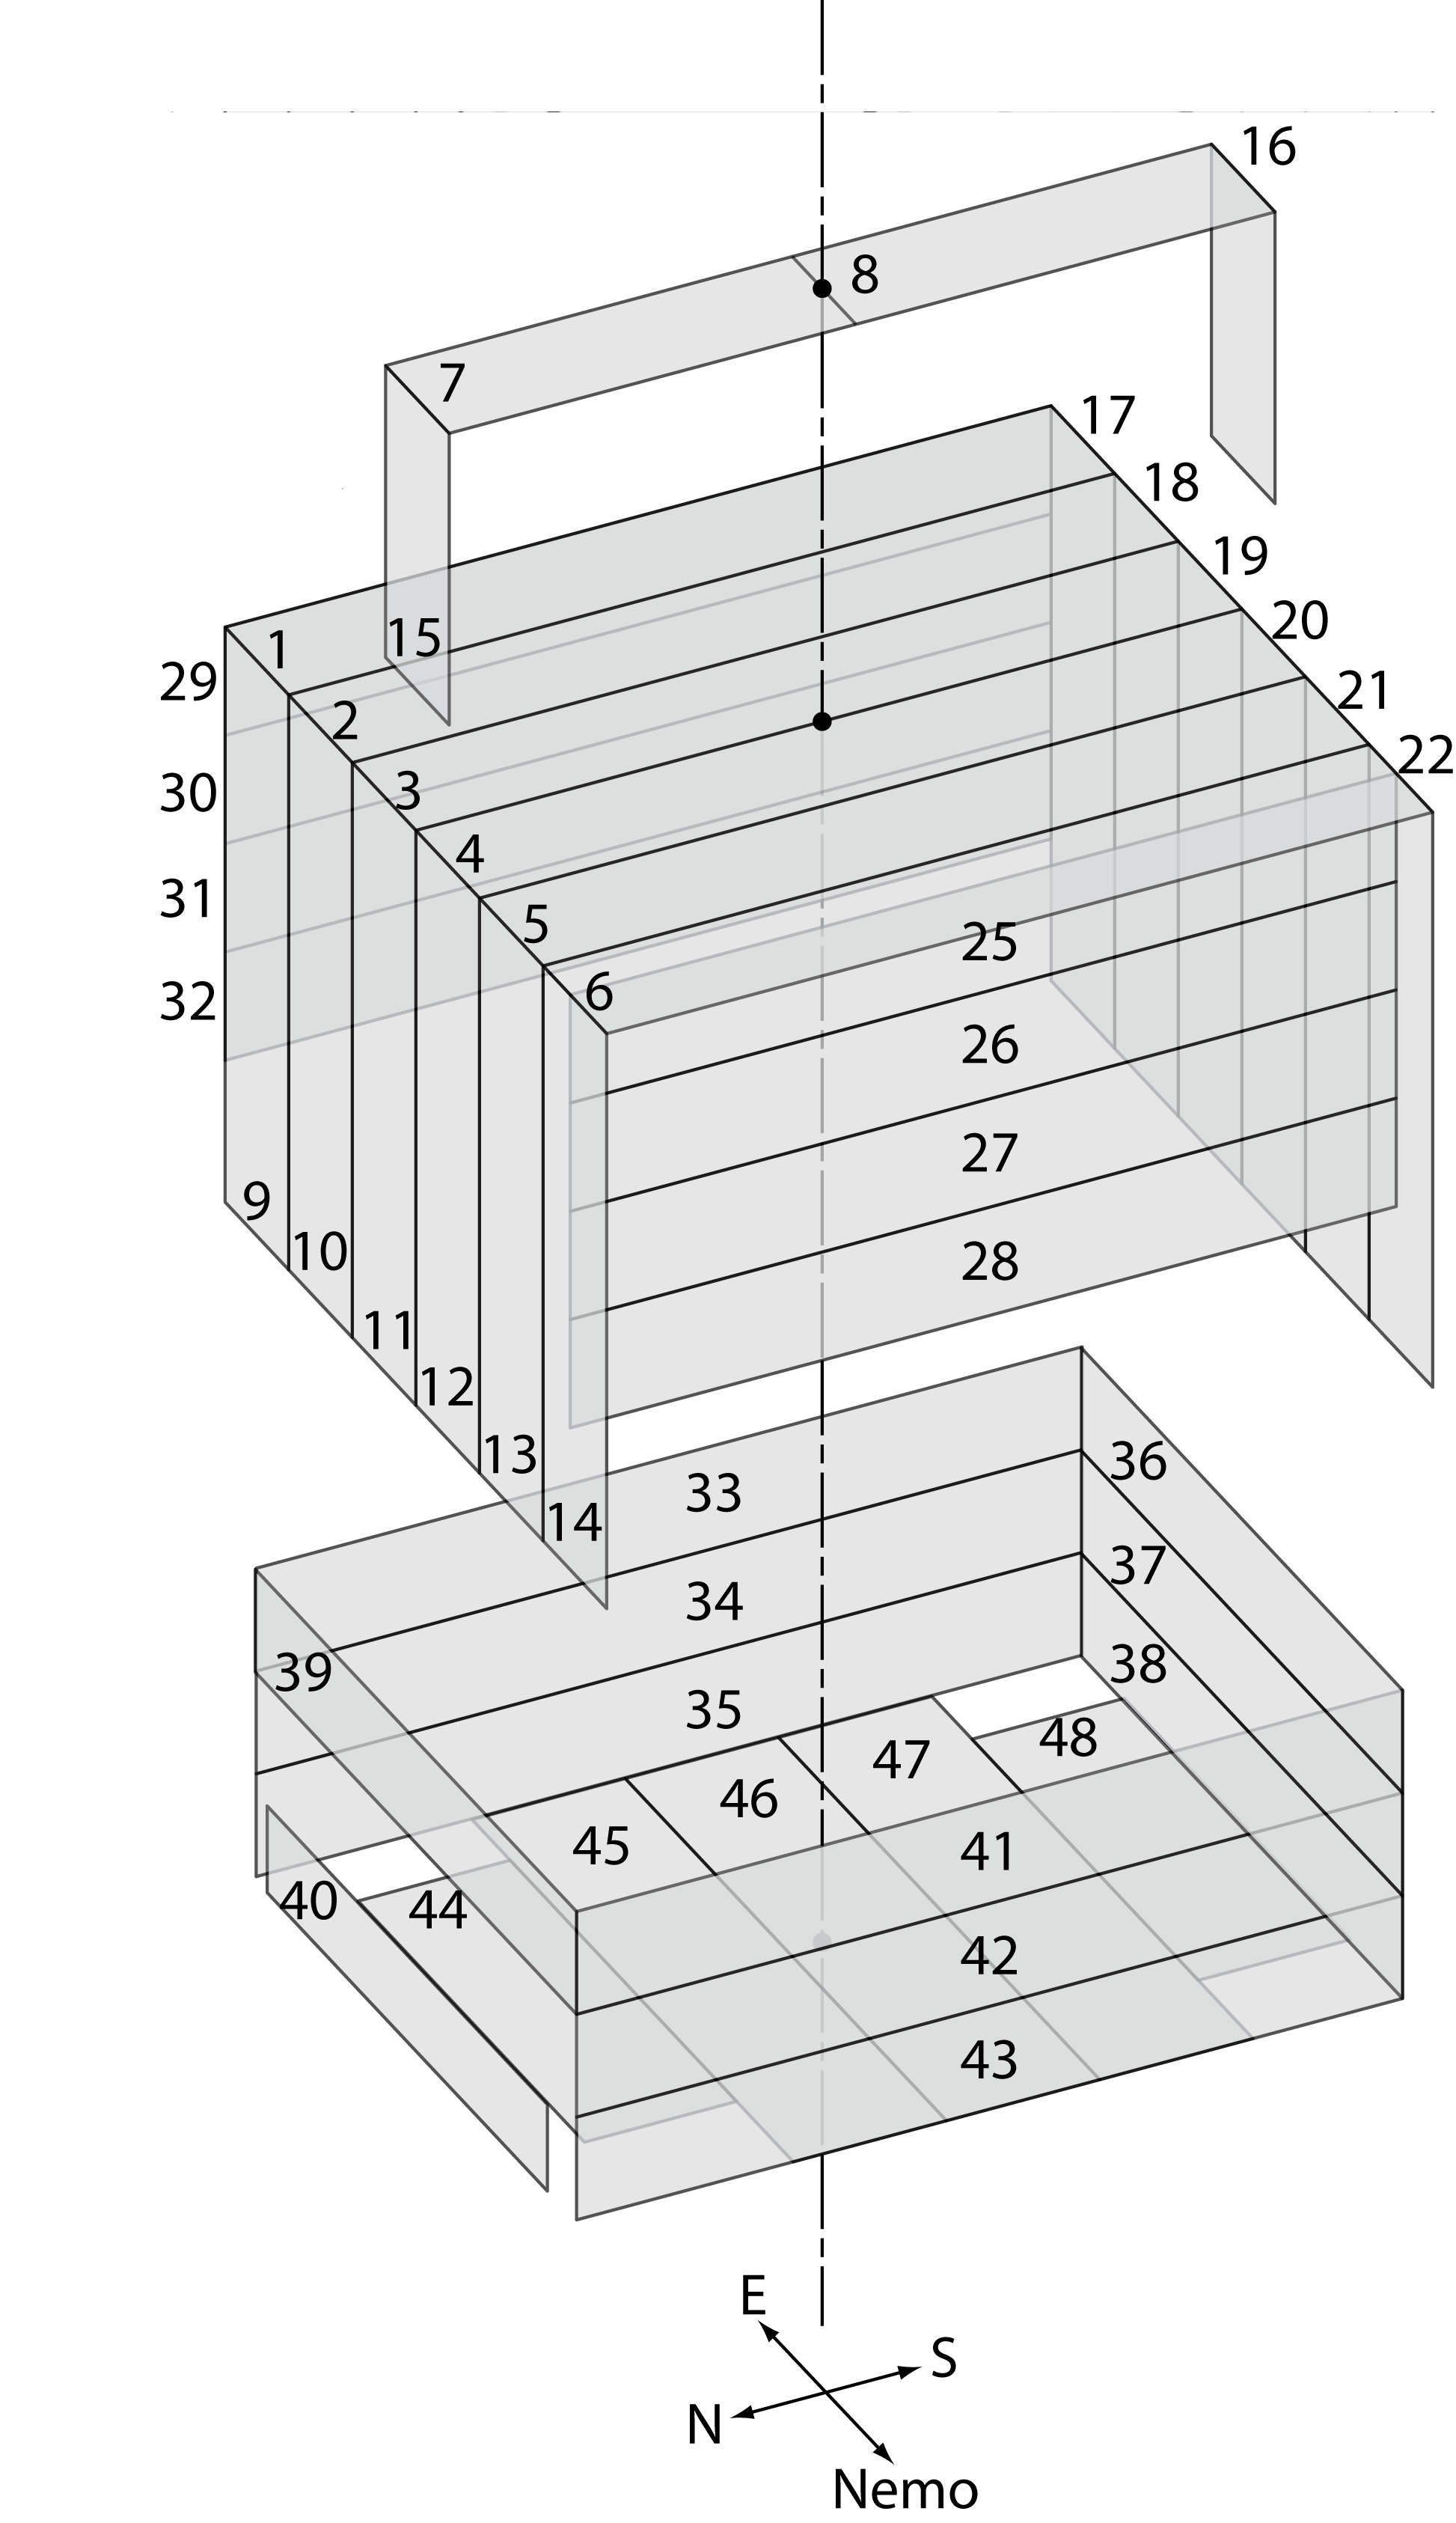
\includegraphics[width=0.5\textwidth{}]{./fig/Veto.png}
  \caption{Schematic view of Muon-Veto System. Each wall of the system is labelled according to its geometric orientation in the laboratory. }.
  \label{fig:muon-setup}
\end{figure}

To cover the gap resulted from the opening of the upper parts, M7, M8, M15 and M16 are installed in 2010. The four extra modules are equipped with LEDs to moniter the stability of the system. M7 and M8 have 3 LEDs along their axis, each of M15 and M16 has one LED installed in the middle. M7 and M8 are $\SI{2.1}{m}$ long. M15 and M16 are around $\SI{1}{m}$ long and cover only partly the opening of upper part.

The other modules have a width of $\SI{65}{cm}$ and a thickness of $\SI{5}{cm}$. Their lengths varies from $\SI{2}{m}$ to $\SI{4}{m}$.
Due to the opening for electronics and the shorter length of some modules, the overall geometric efficiency is 98\%. However, the muon going through the gap can partly be detected via the particle showers induced by them.

A group of four Photomultiplier Tubes (PMT) are installed at each module end. Each PMT group is individually biased with a high voltage (HV). The HV values are set around $\SI{-1500}{V}$ and seldom changed over years to compensate the aging effect of the modules.
To ensure the system is fully closed while operating, two lasers measure the position of two halves of the upper part every 15 minutes. One measures the distance from the western wall to M6, the other from the eastern wall to M8. The gap width is calculated by substracting the two distances.


\section{Working Principle of Muon veto system}
\label{sec:muon-working}
\end{itemize}

\subsection{Muon Energy deposit in the scintillator modules}
The average muon energy at LSM is $<E_{\upmu}>_{\mathrm{LSM}}\approx \SI{260}{GeV}$. The high energy muons deposit ~$\SI{2}{MeV\per\cm}$ in the muon-veto modules according to the Bethe formula. Since the scintillator modules have thickness of 5cm, the muon energy deposit in a module is typically above $\SI{10}{MeV}$. Therefore, the muon events can be separated from the background events with energy deposit normally lower than $\SI{4}{MeV}$, which reduces the deadtime of the experiment.
The stochastic process of muon energy deposit can be described by a Landau distribution \cite{Lan44}. Such distribution is asymmetric and has a long tail towards high energy region. To avoid the contribution of large energy deposit from the long tail, the most probable value (MPV) is usually taken to characterize the distribution.
The total energy deposit of muon is also dependent on its path length in a module. The spectrum is thus smeared due to the different orientation of modules and the angular distribution of muon flux. Most muons at LSM have small zenith angle, therefore the muons deposit minimal energy in top and bottom modules and the track length is of the order of the module thickness.
It is also possible that a muon goes through the edge of a module, which is called a \textit{grazing muon}. In such case, the muon traverses only partly the module thickness and deposits lower energy.

\subsection{Readout electronic chain}
The scintillation photons reflect in the module and are guided to the PMT groups. In a PMT group, the photons are then converted to electrons and amplified to a measurable electric signal. Once the signal amplitude is over the trigger threshold, the signal is integrated in the Analog-to-Digital-Converter (ADC) card to obtain the total energy deposit of muon in a module. At the mean time, the Time-to-Digital-Converter (TDC) card stores the time of the signal. If there is a coincidence of 2 PMT groups within $\SI{100}{ns}$ time window, all non-zero signals of the muon-veto system are stored as one event. After the triggering, there is dead-time of $\tau=\SI{0.16}{ms}$ when no events can be detected. The trigger threshold is set to $\SI{150}{mV}$ to ensure the detection efficiency of low energy events without introducing to much dead-time.

\subsection{Position-dependent light output}
In addition to the fluctuation of the muon energy deposit, the light output is also dependent on the position of the interaction in the scintillator modules. Since the light is guided up to $\SI{4}{m}$ to the PMT group, which is much larger than the attenuation length, the light measured by PMT decreases exponentially with the path length $d$. The relation can be aprroximately determined by the Beer-Lambert law:
\begin{equation}
  I(d)=I_{0}\cdot e^{-\frac{d}{\mathrm{\Lambda}_{\mathrm{eff}}}}
\end{equation}
The $\Lambda_{\mathrm{eff}}$ denotes the effective attenuation length and is a detector specific constant.
The scintillator modules in EDELWEISS were previously used in KARMEN experiment. The effective attenuation length was measured to be $\mathrm{\Lambda} \approx \SI{600}{cm}$ in 1997/1998 \cite{Rei98}. However, the modules has aged since then. Some of the effects are radiation damages and decrease of the transparency.

\begin{figure}[ht!]
  \centering
  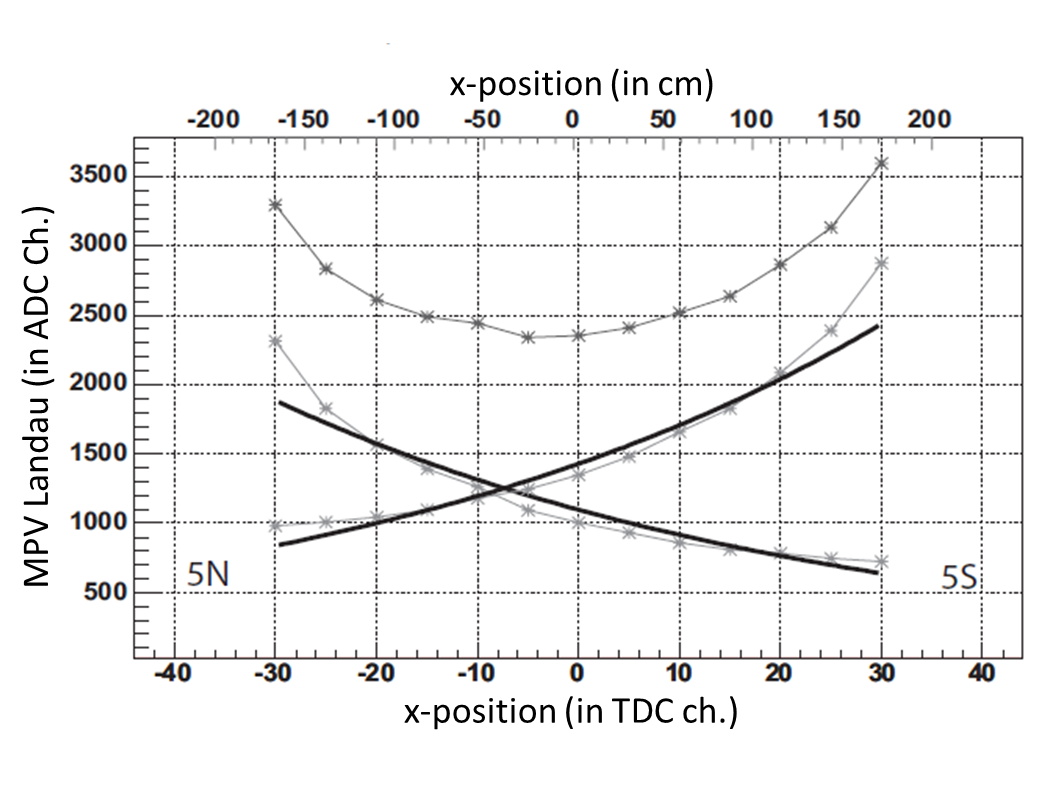
\includegraphics[width=0.6\textwidth{}]{./fig/pos-dependent.png}
  \caption{Light measured in the north and south PMT groups of Module 5 and the sum of them. The data are fitted with exponential curves. Extracted from \cite{Hab04}.}
  \label{fig:pos-dependent}
\end{figure}

In 2003/2004 the attenuation length of two $\SI{4}{m}$ modules were measured. Fig. shows the measured signal in M5 for two individual PMT groups and the sum of them. As shown in the figure, the light yield varies by a factor of 2 from the near end to far end.
For M5 $\Lambda_{\mathrm{eff}}$ was around $\SI{340}{cm}$ and for M1 around $\SI{200}{cm}$ \cite{Hab04}. The measurement shows that the effective attenuation length of scintillator modules has decreased significantly since production, which leads to a decrease of discrimination efficiency for low energy events. This also motivates the importance to analyze the long term stability of the muon-veto system.


\subsection{Available Data of the Muon-Veto Run}

The measured events are stored in data files and combined to so-called Runs. Each Run contains up to 99 files, with each file stores 8 hours measurement. The data in each Run file are converted to a KData file. KData is a ROOT-based \cite{Bru97} data structure and analysis toolkit developed at KIT. It combines the muon-veto data and the bolometer data for coincidence studies \cite{Cox12}.
The data branches relevent in the context of this work and available for the analysis are listed below:
\begin{itemize}
  \item ADC
  When triggered, the integrated signal in each PMT group is stored in ADC units. The HVs of each PMT group are calibrated before the experiment to ensure an uniform gain of each module. Since the modules have aged individually, the correspondence between ADC channels and Energy in MeV varies from module to module. There is also a conversion threshold. For an event with energy deposit under this value, the ADC is not stored and set to -1. The threshold is ~120\,ADC channels and differs from each other.

  \item TDC
  The arrive time of signal in each PMT group is stored. By substracting the two TDC values in one module, the event postion can be reconstructed. In the presented work, the TDC values are only used to probe if a PMT group is triggered.


  \item{PC Time}
  The time of each event are stored in seconds. For the muon-veto events to be compared with bolometer events, an additional timestamp in 10\,\upmu{}s precision is saved. However, such precision is of no interest in analysis of the long term stability. Therefore, the event time in seconds is used in the following analysis.

  \item{DistanceEst,DistanceNemo}
  As described before, the gap size of the upper part of the system is measured every 15 miniutes. DistanceEst stores the distance from eastern wall to M8 and DistanceNemo stores the distance from western wall to M6. For each event, the distances obtained from last laser measurement are saved.

  \item{IsLEDFired}
  The LEDs installed on extra top modules fire every eight hours to monitor the stability of the system. When the event is caused by LED firing, the bool value IsLEDFired will be set to true, allowing a distinction between LED events and other events.
\end{itemize}






%available values
